Este anexo recoge el diseño electrónico de la PCB principal del hexápodo,
desarrollado en Altium Designer, y complementa la descripción funcional del
Capítulo~\ref{cap:hardware}.

% Esta lámina se inserta como imagen para aprovechar la propia página de
% apertura del anexo; \includepdf forzaría un salto y dejaría aquí un gran
% espacio en blanco.
\begin{center}
    \includegraphics[
        page=2,
        width=\textwidth,
        height=0.68\textheight,
        keepaspectratio
    ]{capitulos/anexos/figuras/PCB_HEXAPODO.pdf}
\end{center}

% Expulsamos la página de apertura ANTES de tocar los offsets: así se compone
% con el \hoffset=-1in normal del documento (vmargin) y queda centrada como
% el resto del texto. Si no, el \clearpage interno de \includepdf la
% expulsaría ya con \hoffset=0 y desplazaría título, texto e imagen 1 pulgada
% a la derecha.
\clearpage

% pdfpages no compensa el \hoffset=\voffset=-1in de vmargin y, sin anularlos,
% pegaría la lámina a la esquina superior izquierda. Los ponemos a cero solo
% dentro de este grupo (se restauran al cerrar). Con noautoscale el 0.95 se
% aplica al tamaño real (A4 apaisado) y el giro de 90 grados la deja centrada
% en el centro físico de la hoja.
\begingroup
    \setlength{\hoffset}{0pt}\setlength{\voffset}{0pt}
    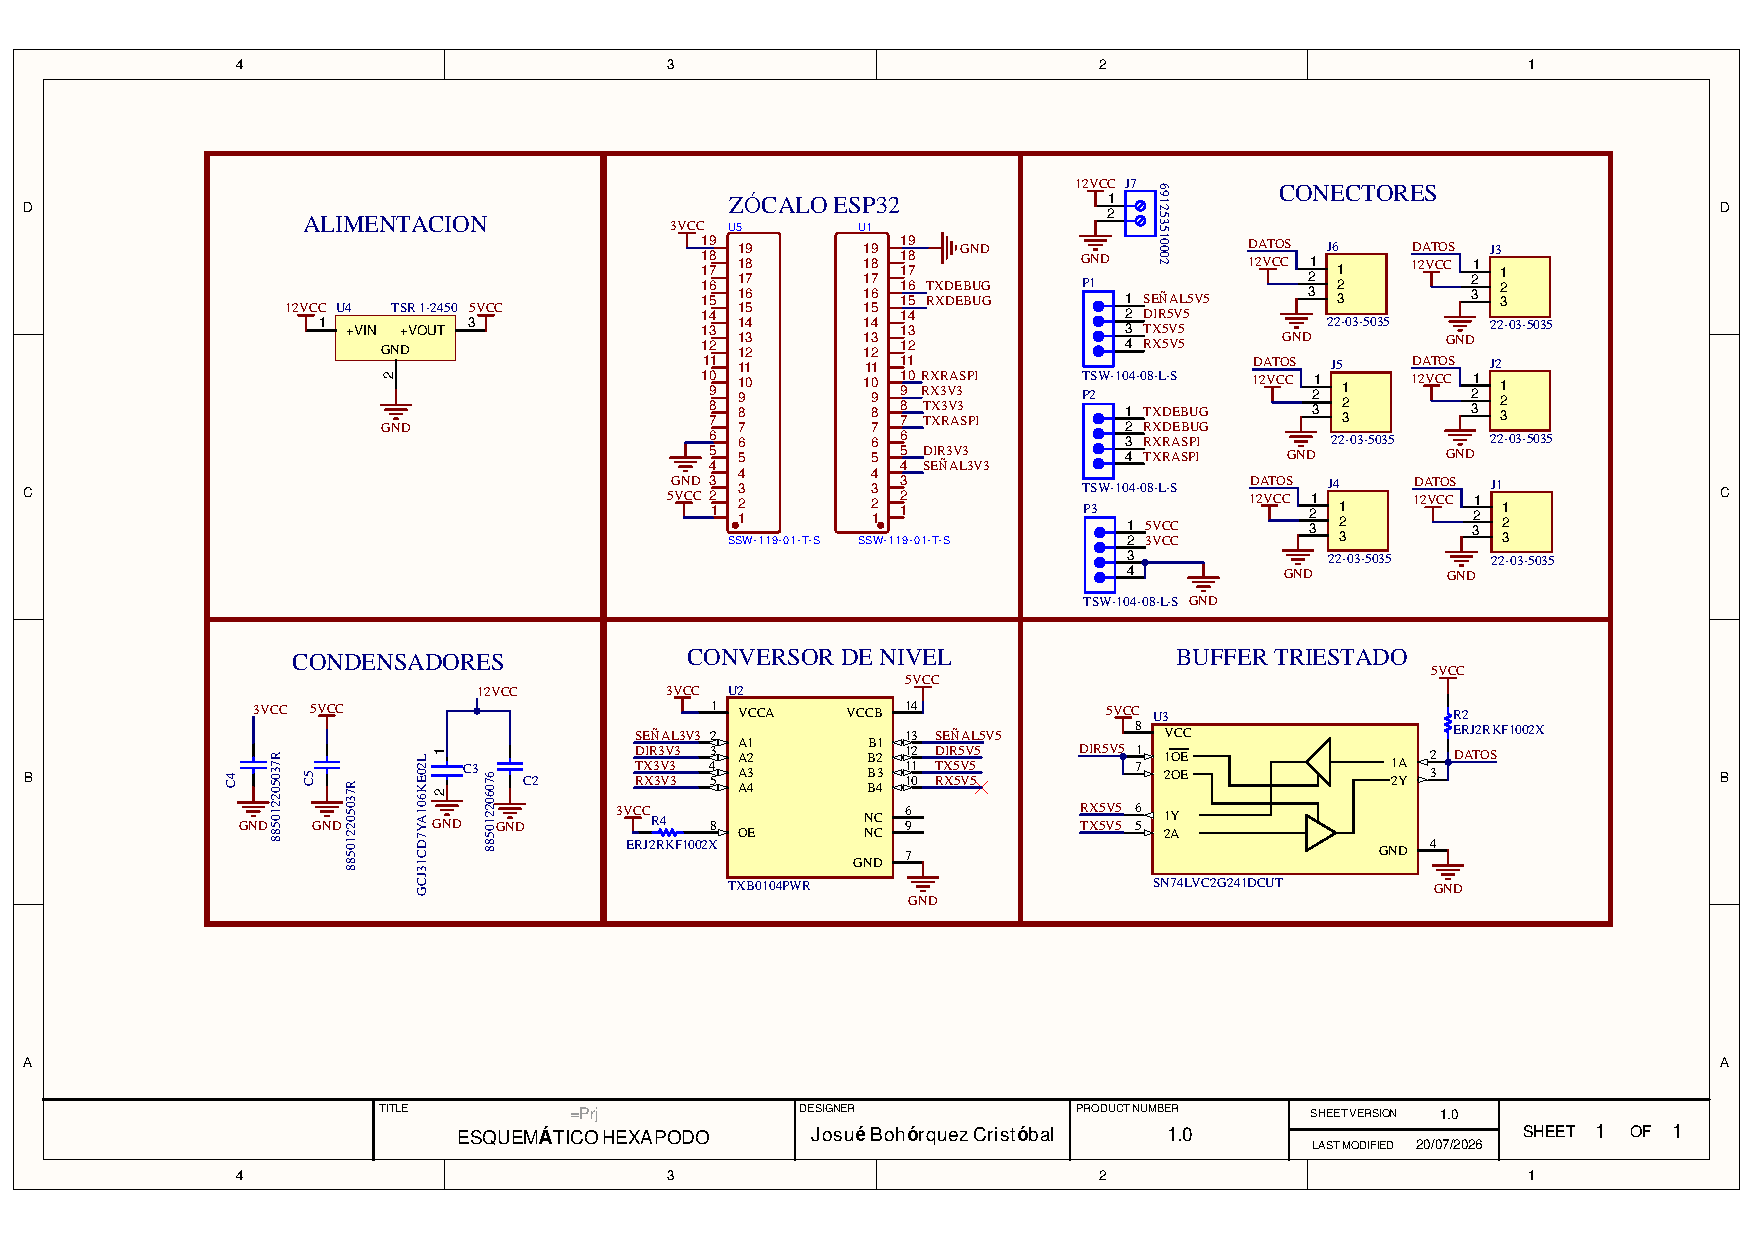
\includepdf[
        pages=1,
        pagecommand={\thispagestyle{empty}},
        angle=90,
        scale=0.95,
        noautoscale=true
    ]{capitulos/anexos/figuras/PCB_HEXAPODO.pdf}
\endgroup
